\documentclass[10pt]{article}

% ----------------------------------------------------------------------------
% CS 59300 midterm report (complete source, ~6 pages excluding figures).
% Figures: fig_dsrl_small.pdf and fig_dsrl_full.pdf must sit next to this file.
% Numbers come from results/*.json, runs/dsrl_small_eideas3/ and
% runs/dsrl_full_eideas3/ in the repository.
% ----------------------------------------------------------------------------

\usepackage[letterpaper,margin=1in]{geometry}
\usepackage[T1]{fontenc}
\usepackage{amsmath}
\usepackage{newtxtext,newtxmath}
\usepackage{booktabs}
\usepackage{graphicx}
\usepackage{enumitem}
\usepackage[hyphens]{url}
\usepackage[colorlinks=true,linkcolor=black,citecolor=black,urlcolor=black]{hyperref}
\usepackage{microtype}

\setlist{itemsep=1pt,topsep=2pt}
\newcommand{\QRLlow}{\underline{Q}_{\mathrm{RL}}}
\newcommand{\QFM}{\tilde{Q}_{\mathrm{FM}}}
\newcommand{\piFM}{\pi_{\mathrm{FM}}}
\newcommand{\piRL}{\pi_{\mathrm{RL}}}
\newcommand{\KL}{\mathrm{KL}}

\title{\textbf{Extracting Q Values from Flow Matching Imitation Policies\\for Online Robot Learning}}
\author{Jialong Ning \and Harshit Moondra \and Zhaopeng Wang \and Karthik Seelam Sreenivas\\[4pt]
\normalsize CS 59300 Midterm Report}
\date{}

\begin{document}
\maketitle

\begin{abstract}
Flow-matching policies model robot actions from demonstrations, but Q2RL-style
value extraction needs likelihood and entropy estimates that their sampling
interface does not provide. We study value estimation from a frozen
flow-matching imitation policy with a conditional arm flow and a categorical
gripper head, whose joint log probability we compute by continuous change of
variables. Combined with policy entropy and a state-value model, it yields an
imitation score for Q-gating against a separate RL policy. As a second route to
online improvement, we steer the frozen flow through its input noise. Frozen
Flow BC succeeds in 60\%, 60\%, and 15\% of episodes on Robomimic Lift, Can, and
Square. In single-seed full-budget runs, latent steering raises success from
46\% to 92\% on Lift and from 52\% to 88\% on Can against BC on the same 50
episodes. On Square, where only 9 of 100 warmup episodes succeed, its critic
diverges and success falls to zero.
\end{abstract}

% ============================================================================
\section{Introduction and research question}

Behavior cloning (BC) fits a conditional action distribution to demonstrations,
and flow matching represents that distribution through a learned velocity
field~\cite{lipman2022flow}. Once deployed, a BC policy keeps sampling from the
same distribution; rewards help only if another mechanism connects them to its
decisions. One option is to train a separate reinforcement-learning (RL) policy
and decide, at each state, whether to execute the imitation or the RL proposal.
Q2RL makes this decision with an imitation value built from policy likelihood,
entropy, and state value~\cite{dodeja2026q2rl}. For a flow policy, these
quantities are absent from the sampling procedure, and the resulting score must
agree with task return well enough to guide selection. We ask:

\begin{quote}\centering\itshape
Can value estimates derived from a frozen flow-matching imitation policy improve
imitation/RL action selection and online sample efficiency over a shared-critic
gate under matched interaction budgets?
\end{quote}

We focus on low-dimensional, single-step manipulation, which keeps density
evaluation tractable and allows a controlled comparison of scoring rules.
Because gating needs both a calibrated score and a competent RL policy, we also
evaluate latent-noise steering~\cite{wagenmaker2025dsrl}, which adapts the same
frozen flow without density queries. Our contributions are (1) a hybrid flow
policy with joint likelihood and entropy estimation and a rollout-based value
model for scoring imitation actions; (2) a matched Q-gating implementation and
protocol that isolate the scoring rule; and (3) a latent-steering learner for
the frozen flow, with a Can pilot and full-budget runs on all three tasks
(Sections~\ref{sec:pilot}--\ref{sec:full}).

% ============================================================================
\section{Related work}

IBRL uses a pretrained imitation policy to propose actions and bootstrap target
values~\cite{hu2024ibrl}; Q2RL builds an imitation action value from an explicit
BC distribution and compares it with a learned RL value~\cite{dodeja2026q2rl}.
Our shared-critic gate is inspired by IBRL. Flow Matching transports a simple
prior to the data distribution~\cite{lipman2022flow}, and FFJORD evaluates
continuous-flow densities through a Jacobian trace with optional Hutchinson
estimation~\cite{grathwohl2018ffjord}; we use these tools and additionally test
calibration against return. ReinFlow~\cite{zhang2025reinflow},
FlowDPG~\cite{shi2026flowdpg}, and Q-VGM~\cite{wang2026qvgm} update the flow
generator itself; we keep it fixed. DSRL instead learns the latent-noise input
of a frozen diffusion or flow policy, with action-to-noise critic
distillation~\cite{wagenmaker2025dsrl}. We reimplement a DSRL-style learner for
our hybrid flow without copying upstream code or claiming exact reproduction.

% ============================================================================
\section{Method}

\subsection{Problem formulation}

We consider a finite-horizon MDP with physical observation $s_k$, action $a_k$,
reward $r_k$, horizon $H$, and $\gamma=0.99$, and maximize
\begin{equation}
  J(\pi) = \mathbb{E}_\pi\Big[\sum_{k=0}^{T-1}\gamma^k r_k\Big], \qquad T\le H.
\end{equation}
The sparse success reward is transformed as $r_k=5r_k^{\mathrm{raw}}-1$ ($-1$
per step, $+4$ on success). Success, termination, or the horizon ends an
episode, so every return lies in $[-100,4]$. Value and RL networks receive
$x_k=(\bar s_k,1-k/H)$ with normalized observation $\bar s_k$; the imitation
policy sees the physical observation only. From demonstrations
$\mathcal{D}=\{(s_i,a_i)\}_{i=1}^N$ we learn a flow policy $\piFM$, fit a
state-value model $V_\psi$ to its rollouts, freeze both, and use their score to
gate a separate actor $\piRL$ with twin critics $Q_{\phi_i}$.

\subsection{Flow matching imitation policy}

An action $a=(b,g)$ has six arm commands $b\in(-1,1)^6$ and a gripper command
$g\in\{-1,0,1\}$. A conditional flow models $b$, and a categorical head
$p_\eta(g\mid s)$ models the sign of the demonstrated gripper command; the two
are conditionally independent given state. With
$u_1=\operatorname{atanh}((1-\epsilon)b)$, $\epsilon=0.001$,
$u_0\sim\mathcal{N}(0,I_6)$, $t\sim\mathcal{U}[0,1]$ and
$u_t=(1-t)u_0+tu_1$, the BC loss is
\begin{equation}
  \mathcal{L}_{\mathrm{BC}} =
  \mathbb{E}\Big[\tfrac{1}{6}\big\|v_\theta(u_t,t\mid s)-(u_1-u_0)\big\|_2^2\Big]
  - \mathbb{E}\big[\log p_\eta(g\mid s)\big].
\end{equation}
At inference we integrate $du_t/dt=v_\theta(u_t,t\mid s)$ from noise with 16
RK4 steps and output $b=\tanh(u_1)$, with no clipping. The velocity network has
two 128-unit SiLU layers and bounded output $6\tanh(v^{\mathrm{raw}}/6)$. We
write $f(s,z)$ for the deterministic map from base noise $z=u_0$ to the arm
command.

\subsection{Likelihood and entropy estimation}

To score a command, we invert the tanh and integrate the flow backward to its
base point. Continuous change of variables gives
\begin{equation}
  \log\piFM(b,g\mid s) = \log p_0(u_0)
  - \int_0^1 \nabla_u\!\cdot v_\theta(u_t,t\mid s)\,dt
  - \sum_{j=1}^{6}\log\big(1-b_j^2\big) + \log p_\eta(g\mid s),
\end{equation}
a mixed density with Lebesgue measure for the arm and counting measure for the
gripper. The divergence uses the exact trace or a fixed-probe Hutchinson
estimate. Entropy is estimated from $M=8$ samples, in nats:
\begin{equation}
  \hat{\mathcal{H}}(s) = -\frac{1}{M}\sum_{m=1}^{M}\log\piFM\big(a^{(m)}\mid s\big),
  \qquad a^{(m)}\sim\piFM(\cdot\mid s).
\end{equation}

\subsection{Value estimation from the frozen policy}

We fit $V_\psi(x_k)$ to Monte Carlo returns $G_k=\sum_{j\ge k}\gamma^{j-k}r_j$ of
complete BC rollouts. Failed episodes keep their actual finite returns, unlike
the Q2RL code's $r_{\mathrm{neg}}/(1-\gamma)$ shortcut. Following Q2RL,
\begin{equation}
  \QFM(x,a) = V_\psi(x) + \alpha_Q\big[\log\piFM(a\mid s) + \hat{\mathcal{H}}(s)\big].
  \label{eq:qfm}
\end{equation}
The bracket has zero mean under $\piFM$, but reading it as an advantage assumes
the policy is roughly Boltzmann in the task Q-function, so its calibration and
ranking must be measured. The RL actor and critics are initialized from the
collected BC actions and frozen scores, and both gating conditions share these
artifacts.

\subsection{Online reinforcement learning and Q gating}

The RL actor has a tanh-Gaussian arm head and a categorical gripper head. Twin
critics use the target
\begin{equation}
  y = r + \gamma(1-d)\min_i Q_{\bar\phi_i}(x',a'), \qquad a'\sim\piRL(\cdot\mid x'),
\end{equation}
without entropy, and the actor minimizes
$\mathbb{E}[\alpha_{\mathrm{SAC}}\log\piRL(a\mid x)-\min_iQ_{\phi_i}(x,a)]$ with
$\alpha_{\mathrm{SAC}}=0.01$, separate from $\alpha_Q=1$. At each step, with
$\QRLlow=\min_iQ_{\phi_i}$ and $a_{\mathrm{RL}}$ the actor's mode, the gate
executes
\begin{equation}
  a_k = \begin{cases}
    a_{\mathrm{RL}}, & \QRLlow(x_k,a_{\mathrm{RL}}) > \QFM(x_k,a_{\mathrm{FM}}),\\
    a_{\mathrm{FM}}, & \text{otherwise.}
  \end{cases}
\end{equation}
Every executed transition enters replay. The shared-critic gate replaces
$\QFM(x,a_{\mathrm{FM}})$ with $\QRLlow(x,a_{\mathrm{FM}})$.

\subsection{Latent steering of the frozen flow}
\label{sec:latent}

Latent steering learns $\pi_Z(z\mid x)=\mathcal{N}(\mu_\omega(x),\sigma_\omega(x)^2)$
over the arm noise and executes $(f(s,z),g)$ with $g\sim p_\eta$. Following
DSRL's noise-aliasing variant~\cite{wagenmaker2025dsrl}, twin action critics
learn from executed transitions with
\begin{equation}
  y = r + \gamma(1-d)\,\mathbb{E}_{g'\sim p_\eta}\Big[\min_i Q^A_{\bar\phi_i}\big(x',(f(s',z'),g')\big)\Big],
  \qquad z'\sim\pi_Z(\cdot\mid x').
\end{equation}
A noise critic $Q^Z$ is distilled at replay states, from latents drawn half from
the prior and half from $\pi_Z$, toward
$\mathbb{E}_g[\min_iQ^A_i(x,(f(s,z),g))]$ with the flow and teacher detached, so
no inverse flow or latent labels are needed. The steering policy minimizes
\begin{equation}
  \mathbb{E}_{z\sim\pi_Z}\big[-\min_i Q^Z_i(x,z)\big]
  + \beta\,\KL\big(\mathcal{N}(\mu_\omega,\sigma_\omega^2)\,\big\|\,\mathcal{N}(0,I)\big),
\end{equation}
with $\mu_\omega=2\tanh(\cdot)$ and $\sigma_\omega\le1$. It starts at exactly
$\mathcal{N}(0,I)$, so it initially reproduces BC. Critic targets decode with 8
RK4 steps and executed actions with 16 (maximum action difference
$1.1\times10^{-3}$ on Lift replay states, 1.8$\times$ faster updates). Because
ODE-plus-tanh is injective, the benefit of action-to-noise distillation must be
measured rather than assumed.

% ============================================================================
\section{Evaluation protocol}

\paragraph{Tasks.}
We use the proficient-human demonstrations of Robomimic Lift, Can, and
Square~\cite{mandlekar2021matters} (\texttt{low\_dim\_v141.hdf5} from the
official Q2RL mirror at a fixed revision) with the train/validation masks
verified from the released Q2RL checkpoints (Table~\ref{tab:splits}). A Panda
robot is controlled at 20\,Hz by single-step relative OSC\_POSE commands
($\pm1$ maps to $\pm0.05$\,m and $\pm0.5$\,rad). Observations are end-effector
pose, gripper joint positions, and object features, normalized with training
statistics and a 0.02 standard-deviation floor.

\begin{table}[t]
  \centering\small
  \caption{Demonstration splits and task settings.}
  \label{tab:splits}
  \begin{tabular}{lrrrr}
    \toprule
    Task & State dim. & Train / valid demos & Train / valid transitions & $H$ \\
    \midrule
    Lift   & 19 & 36 / 4   & 1{,}769 / 223     & 300 \\
    Can    & 23 & 180 / 20 & 20{,}883 / 2{,}324 & 300 \\
    Square & 23 & 180 / 20 & 27{,}165 / 2{,}989 & 500 \\
    \bottomrule
  \end{tabular}
\end{table}

\paragraph{Conditions.}
Table~\ref{tab:conditions} lists the online conditions. B and C share the frozen
policy, warmup data, and initialization, so they differ only in the imitation
score; an ungated RL condition is planned. D adapts the same policy by latent
steering. Relative to the Q2RL reference, we use twin 128-unit critics instead
of a 10-member 512-unit ensemble, no BC auxiliary actor loss, sparse evaluation
reward, and MuJoCo 3.2.6 instead of 3.1.6, so we do not claim a reproduction.

\begin{table}[t]
  \centering\small
  \caption{Online conditions on the same frozen flow. All four are implemented.}
  \label{tab:conditions}
  \begin{tabular}{llll}
    \toprule
    Condition & Imitation score & RL score & Executed action \\
    \midrule
    A: Frozen Flow BC      & --                              & --                              & Always imitation \\
    B: Shared-critic gate  & $\QRLlow(x,a_{\mathrm{FM}})$    & $\QRLlow(x,a_{\mathrm{RL}})$    & Higher score \\
    C: Flow-derived gate   & $\QFM(x,a_{\mathrm{FM}})$       & $\QRLlow(x,a_{\mathrm{RL}})$    & Higher score \\
    D: Latent steering     & --                              & $Q^Z(x,z)$                      & $(f(s,z),g)$, $z\sim\pi_Z$ \\
    \bottomrule
  \end{tabular}
\end{table}

\paragraph{Settings.}
BC uses 10{,}000 Adam updates (batch 256, learning rate $3\times10^{-4}$). The
gating runs use 100 BC warmup episodes, 20{,}000 initialization updates (50{,}000
for Square), one update per transition, and up to 500{,}000 interactions; we
plan three RL seeds per BC checkpoint and 50 paired evaluation episodes.
Latent steering uses 100 warmup episodes, 1{,}500 pretraining updates, then
$10^5$ online steps at 20 updates per step (2{,}001{,}500 updates), batch 128,
$\beta=3$, and evaluates BC and the steered policy on the same 50 reset seeds
every $10^4$ steps. Warmup counts toward the budget; evaluation interactions are
counted separately and never enter replay. On CPU nodes of Purdue's Gilbreth
cluster a learner update took about 0.05\,s, so we run learners in float64 on a
workstation with two RTX~5080 GPUs, keeping simulation and seeded noise on the
CPU so paired evaluations match a CPU run.

\paragraph{Metrics.}
We report success against training interactions, area under the success curve,
and interactions needed to exceed BC, with seed variation separated from
binomial uncertainty. Paired seeds also let us count episodes solved by only one
policy. To test Eq.~\eqref{eq:qfm}, we will restore simulator snapshots, execute
a chosen first action, and continue with BC to estimate $Q^{\piFM}(x,a)$ for
bias and ranking, with ablations over 16--64 integration steps, exact versus
Hutchinson traces, and entropy sample counts.

% ============================================================================
\section{Preliminary results}

The gating conditions are implemented but not yet run, so we report BC, flow
checks, and latent steering.

\subsection{Frozen Flow BC}

Each task was trained once (seed 0) and evaluated frozen on 20 reset seeds
(Table~\ref{tab:bc}). Lift and Can succeed in 12/20 episodes and Square in 3/20.
Lift's validation loss is far above its training loss and was lowest at update
3{,}001 (0.329), so it overfits its 36 demonstrations and the final iterate is
not the best checkpoint. Square's low loss does not give reliable control.
Sampling costs about 3.2\,ms per step on a CPU.

\begin{table}[t]
  \centering\small
  \caption{Frozen Flow BC, one training seed, 20 evaluation episodes per task.}
  \label{tab:bc}
  \begin{tabular}{lrrrr}
    \toprule
    Task & Success & 95\% Wilson CI & Train / valid loss & ms / step \\
    \midrule
    Lift   & 12/20 (60\%) & [0.39, 0.78] & 0.203 / 0.955 & 3.29 \\
    Can    & 12/20 (60\%) & [0.39, 0.78] & 0.510 / 0.480 & 3.18 \\
    Square &  3/20 (15\%) & [0.05, 0.36] & 0.377 / 0.457 & 3.22 \\
    \bottomrule
  \end{tabular}
\end{table}

\subsection{Numerical checks}

Encoding and decoding seeded noise at eight fixed states per task gives a
maximum round-trip error of at most $2.0\times10^{-4}$ at 16 RK4 steps and below
$2\times10^{-7}$ at 64. All 17 unit tests pass on the GPU machine, including
analytic density and entropy tests and CUDA--CPU agreement. On a synthetic
two-mode flow with one rewarded mode, steering raises the rewarded fraction from
0.506 to 0.99.

\subsection{Latent-steering pilot on Can}
\label{sec:pilot}

From a shared buffer of 50 BC warmup episodes (33 successful), run C trained
offline (4{,}000 updates) and runs D and E added 5{,}000 online steps at 5
updates per step with $\beta=3$ (D) or $\beta\in\{1,10\}$ (E), on a Can flow
retrained on the GPU machine (12/20 BC success on seeds 40000--40019). The
untrained steering policy reproduced BC exactly. With $\beta=3$, success rose
from 60\% to 75\% with no episode lost to BC (Table~\ref{tab:pilot},
Figure~\ref{fig:pilot}); $\beta=1$ drifted below BC and $\beta=10$ barely moved
(KL $4\times10^{-4}$). With 20 episodes, the interval for 15/20, [0.53, 0.89],
still overlaps BC's.

\begin{table}[t]
  \centering\small
  \caption{Latent-steering pilot on Can, 20 paired episodes; BC succeeds in 12/20
  at every evaluation. Last two columns count episodes at 5{,}000 steps solved by
  only one policy.}
  \label{tab:pilot}
  \begin{tabular}{llrrrr}
    \toprule
    Run & Setting & 2{,}500 steps & 5{,}000 steps & Steered only & BC only \\
    \midrule
    C & offline, $\beta=3$ & \multicolumn{2}{c}{12/20 (no online steps)} & 1 & 1 \\
    D & online, $\beta=3$  & 12/20 & \textbf{15/20} & 3 & 0 \\
    E & online, $\beta=1$  & 14/20 & 11/20 & 2 & 3 \\
    E & online, $\beta=10$ & 13/20 & 13/20 & 1 & 0 \\
    \bottomrule
  \end{tabular}
\end{table}

\begin{figure}[t]
  \centering
  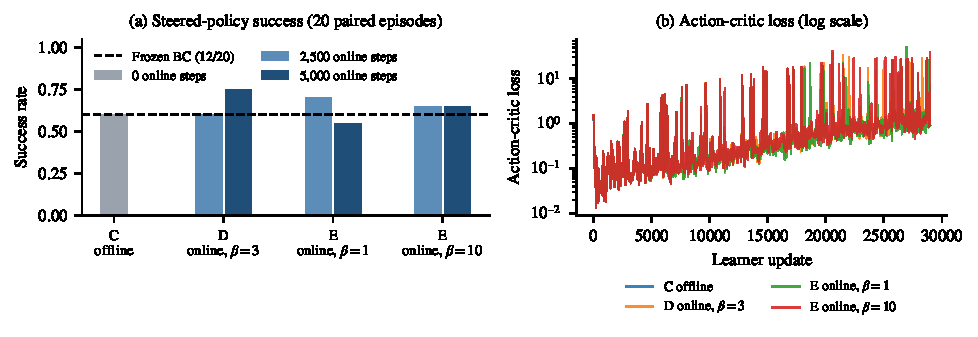
\includegraphics[width=\linewidth]{fig_dsrl_small.pdf}
  \caption{Latent-steering pilot on Can. (a) Steered success at each evaluation;
  dashed line is BC on the same seeds. (b) Action-critic loss, every 50 updates.}
  \label{fig:pilot}
\end{figure}

\subsection{Full-budget latent steering}
\label{sec:full}

We then ran the full budget on all three tasks with $\beta=3$ and one training
seed. The runs took 13.6--19.6 hours with 22--28\,ms updates, and the flow
weights were unchanged afterward. BC was re-measured on the same 50 seeds
(40000--40049) used for the steered policy (Table~\ref{tab:full}).

\begin{table}[t]
  \centering\small
  \caption{Full-budget latent steering, one training seed, $\beta=3$, 50 paired
  episodes every $10^4$ online steps, with 95\% Wilson intervals. Last two
  columns count final-evaluation episodes solved by only one policy.}
  \label{tab:full}
  \setlength{\tabcolsep}{4pt}
  \begin{tabular}{lrrrrrrr}
    \toprule
    Task & Warmup wins & BC & Steered, $10^4$ & Steered, final & Best & Steered only & BC only \\
    \midrule
    Lift   & 51/100 & 23/50 [0.33, 0.60] & 43/50 & \textbf{46/50} [0.81, 0.97] & 48/50 & 23 & 0 \\
    Can    & 61/100 & 26/50 [0.39, 0.65] & 39/50 & \textbf{44/50} [0.76, 0.94] & 44/50 & 18 & 0 \\
    Square &  9/100 &  4/50 [0.03, 0.19] &  5/50 & 0/50 [0.00, 0.07]          &  5/50 &  0 & 4 \\
    \bottomrule
  \end{tabular}
\end{table}

On Lift and Can, steering beats BC at all ten evaluations and the final
intervals do not overlap BC's. Most of the gain arrives in the first $10^4$
steps (Figure~\ref{fig:full}a). At the end, the steered policy solves 23 Lift
and 18 Can episodes that BC fails and loses none, and its successes are shorter
(42 vs.\ 55 steps on Lift, 111 vs.\ 119 on Can).

Square fails through critic divergence. With 9 successful warmup episodes among
about 47{,}000 transitions, the steered policy stays near BC for 60{,}000 online
steps and then solves no episode from 70{,}000 onward. Since true values lie in
$[-100,4]$, the mean TD target leaving that range at 1.28 million updates
(about 64{,}000 steps) and ending near $-10^3$ marks divergence
(Figure~\ref{fig:full}b). The late action-critic loss median is about $10^4$
(2.7 on Can), the late KL median 2.4 (0.014 on Can), latent means hit the
$\pm2$ bound, and the smallest latent standard deviation falls to 0.007. Lift's
TD target also settles slightly out of range, near $-125$, without hurting
success. Sparse successes with 20 updates per step appear to destabilize the
critic.

\begin{figure}[t]
  \centering
  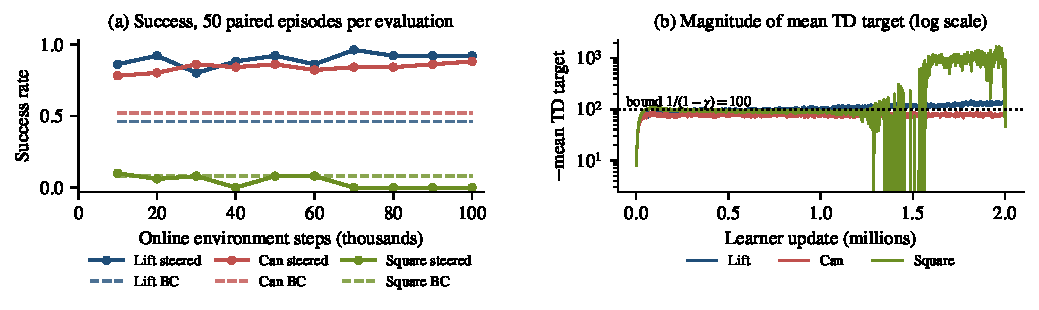
\includegraphics[width=\linewidth]{fig_dsrl_full.pdf}
  \caption{Full-budget latent steering, one seed. (a) Steered (solid) and BC
  (dashed) success against online steps after warmup. (b) Magnitude of the mean
  TD target; the dotted line is the largest magnitude a true value can reach.}
  \label{fig:full}
\end{figure}

% ============================================================================
\section{Remaining plan}

We will complete held-out score calibration and a bounded B/C pilot, then run
matched gating comparisons with the ungated condition and a small $\alpha_Q$
sweep on the same GPU setup. For latent steering, we will add at least two seeds
on Lift and Can and rerun Square with TD targets bounded to $[-100,4]$, fewer
updates per step, and demonstrations in replay. Validation-based checkpoint
selection will be examined before fixing the BC policies, especially for Lift.
Table~\ref{tab:plan} assigns the work. The main risk is that BC density is
accurate but poorly calibrated to return; the fallback is a focused study of
where calibration and ranking break down, with the shared-critic gate as
control. If density queries are too slow, we will test Hutchinson estimation or
a density surrogate. Lift and Can take priority if Square proves impractical.

\begin{table}[t]
  \centering\small
  \caption{Remaining work and responsibility assignments.}
  \label{tab:plan}
  \begin{tabular}{lll}
    \toprule
    Work package & Deliverable & Owner \\
    \midrule
    BC and data            & Fixed checkpoints, split verification, checkpoint selection & \textit{[Name]} \\
    Value estimation       & Return calibration, ranking, density-cost study             & \textit{[Name]} \\
    Online comparisons     & Matched gating runs and ungated RL condition                & \textit{[Name]} \\
    Latent steering        & Additional seeds, Square stabilization, $\beta$ sensitivity & \textit{[Name]} \\
    Evaluation and writing & Seed statistics, figures, failure analysis, final report    & \textit{[Name]} \\
    \bottomrule
  \end{tabular}
\end{table}

% ============================================================================
\begin{thebibliography}{9}\small
\setlength{\itemsep}{0pt}

\bibitem{dodeja2026q2rl}
L.~Dodeja et~al.
\newblock When Life Gives You {BC}, Make {Q}-functions: Extracting {Q}-values
  from Behavior Cloning for On-Robot Reinforcement Learning.
\newblock RSS, 2026. arXiv:2605.05172v3.

\bibitem{hu2024ibrl}
H.~Hu, S.~Mirchandani, and D.~Sadigh.
\newblock Imitation Bootstrapped Reinforcement Learning.
\newblock RSS, 2024. arXiv:2311.02198.

\bibitem{lipman2022flow}
Y.~Lipman, R.~T.~Q. Chen, H.~Ben-Hamu, M.~Nickel, and M.~Le.
\newblock Flow Matching for Generative Modeling.
\newblock 2022. arXiv:2210.02747.

\bibitem{grathwohl2018ffjord}
W.~Grathwohl, R.~T.~Q. Chen, J.~Bettencourt, I.~Sutskever, and D.~Duvenaud.
\newblock {FFJORD}: Free-form Continuous Dynamics for Scalable Reversible
  Generative Models.
\newblock 2018. arXiv:1810.01367.

\bibitem{zhang2025reinflow}
T.~Zhang, C.~Yu, S.~Su, and Y.~Wang.
\newblock {ReinFlow}: Fine-tuning Flow Matching Policy with Online
  Reinforcement Learning.
\newblock NeurIPS, 2025. arXiv:2505.22094.

\bibitem{shi2026flowdpg}
K.~Shi et~al.
\newblock {FlowDPG}: Deterministic Policy Gradient on Flow Matching Policies
  for Real-World Manipulation.
\newblock 2026. arXiv:2606.22303v2.

\bibitem{wang2026qvgm}
Z.~Wang et~al.
\newblock {Q-VGM}: {Q}-Guided Value-Gradient Matching for Offline-to-Online
  {RL} of Flow-Matching {VLA} Policies.
\newblock 2026. arXiv:2606.08015v5.

\bibitem{wagenmaker2025dsrl}
A.~Wagenmaker et~al.
\newblock Steering Your Diffusion Policy with Latent Space Reinforcement
  Learning.
\newblock 2025. arXiv:2506.15799v2.

\bibitem{mandlekar2021matters}
A.~Mandlekar et~al.
\newblock What Matters in Learning from Offline Human Demonstrations for Robot
  Manipulation.
\newblock CoRL, 2021. arXiv:2108.03298.

\end{thebibliography}

\end{document}
